\documentclass[10pt]{article}

\usepackage[utf8]{inputenc}
\usepackage{amssymb}
\usepackage{enumitem}
\usepackage{longtable}
\usepackage{nopageno}
\usepackage{float}
\usepackage{placeins}

\usepackage{subfig}
\usepackage{graphicx}
\graphicspath{{./images/}}

\usepackage{rotating}
\def\rot{\rotatebox}

\usepackage{url}
\usepackage{hyperref}
\hypersetup{colorlinks=true, linkcolor=black, filecolor=magenta, urlcolor=blue,
    citecolor=black}

\usepackage[normalem]{ulem}
\useunder{\uline}{\ul}{}
\usepackage{multirow}

\usepackage{geometry}
\geometry{
 a4paper,
 total={170mm,257mm},
 left=10mm,
 right=10mm,
 top=10mm,
 bottom=10mm,
}


\begin{document}


\begin{center}
    \Huge\textbf{CS261 Coursework Design Document}\\
    \vspace{2mm}
    \large{\textit{\textbf{Group 17:} Ben Lewis, Dan Risk, Edmund Goodman,
    Jay Re Ng, John-Loong Gao, Rahul Vanmali, Tomás Chapmann Fromm}}
\end{center}


\section{Introduction}
% \vspace{-6mm}\section{Introduction}\vspace{-2mm}
Deutsche Bank requires a system prototype to support the mentoring process for
employees. The principal purpose of this document is to broadly record the
process documentation and design choices for said system prototype. For process
documentation, this document will detail development methodologies in addition
to workflow and project organisation. Design choices include a prototype user
interface design and technical diagrams demonstrating user interactions between
multiple users and the system. Furthermore, our testing strategy and technical
descriptions such as choice of technologies used and system architecture will be
covered in depth to illustrate a fuller idea of the final product.

\section{Process documentation and planning}
\subsection{Development methodology}
We opted for an agile development methodology based on the Scrum model. The
development timeline will be broken down into a large initial planning phase and
a series of week-long sprints. We chose to elect our project manager as scrum
master, since this role is similar to that of the project manager in organising
the team and improving workflow. We will use Trello to create and manage a scrum
board, which will allow for easy management of the product backlog. At the start
of each sprint, we will meet to discuss the items from the product backlog to be
completed in that sprint - this will usually be decided according to the project
timeline below, however some small adaptations may need to be made. Each day
within the sprint, the team will discuss progress and bring to attention any
challenges they are facing. At the end of the sprint, we will carry out a sprint
review, and each developer can showcase parts of the system which have been
completed. The sprint cycle is completed with a sprint retrospective, where
improvements can be made to the development process before the next sprint.

An agile methodology is optimal for a short timeframe as it allows rapid product
development with concurrent implementation and testing so we can make effective
use of the time available. It also allows for more flexibility if we face
unexpected delays during development, which is likely with an inexperienced
team. Producing a thorough plan before beginning the agile development process
is suitable since deliverable deadlines are fixed, so ensuring work is completed
on time is critical. Additionally, contact with the client is limited so
requirements are unlikely to change and the project will not deviate much from
the initial plan.


\subsection{Project organisation and communication}
We decided on a flat team hierarchy since we have similar levels of software
development experience, self-managed but with well defined responsibilities. To
communicate between meetings, we decided to use Discord, as it is already a
popular choice within the team and is easy to learn for new users. It offers
both text and voice chat as well as a number of features such as GitHub
integration, so we are notified via Discord when pull requests are made, for
example.

Discord can be used for online meetings however we aim to convene in-person at
least twice a week, as this enables us to share ideas much more easily and
maintain focus during meetings. At these meetings we can compare progress on the
system with our plan, and assign tasks based on documentation or what tasks need
doing in order to stay on schedule. We will use Trello to manage the product
backlog, and see which tasks are currently in progress, to ensure the project
will be completed by the deadline.

\subsection{Risk management}
% \begin{table}[]
\begin{longtable}{|p{0.105\linewidth}|p{0.15\linewidth}|p{0.075\linewidth}|p{0.06\linewidth}|p{0.175\linewidth}|p{0.15\linewidth}|p{0.06\linewidth}|}
\hline \rot{45}{\textbf{Risk}} & \rot{45}{\textbf{Impact}} & \rot{45}{\textbf{Likelihood}} & \rot{45}{\textbf{Severity}} & \rot{45}{\textbf{Mitigation}} & \rot{45}{\textbf{Contingency}} & \rot{45}{\textbf{Residual}} \\ \hline\hline
    Team members unable to work & Smaller team until the member can resume work                     & 2 & 7 & Team members take precautions                                 & Reduce scope and reallocate work across team  & 2 \\ \hline
    Task longer than expected   & Project delayed until task completed                              & 5 & 4 & Allocate buffer time to allow overrunning tasks               & Re-assign team members to load balance        & 4 \\ \hline
    Poor code quality           & System fails testing or linting procedures                        & 5 & 4 & Code review and automated testing through CI/CD               & Re-assign team memebrs to fix pair program    & 3 \\ \hline
    Requirements change         & Design and existing code must be changed                          & 3 & 8 & Use an agile methodology to facilitate requirements change    & Update project plan and proceed with new one  & 3 \\ \hline
    Code lost                   & Code must be re-written                                           & 1 & 7 & Use `git` as version control, and remote backup to GitHub     & Restore code from local or remote backups     & 1 \\ \hline
    Problems with dependencies  & Component of project fails external library or technology         & 2 & 4 & Choose technologies and dependencies carefully                & Find replacement library or technology        & 2 \\ \hline
    Scope creep                 & Addition of unnecessary features causing growth of project scale  & 7 & 4 & Include extra features in project timeline, and stick to it   & Drop lowest priority features                 & 5 \\ \hline
    \caption{The risk register, for our project}
    \label{tab:risk_table}
\end{longtable}

\subsection{Project schedule}
\begin{figure}[H]
    \centering
    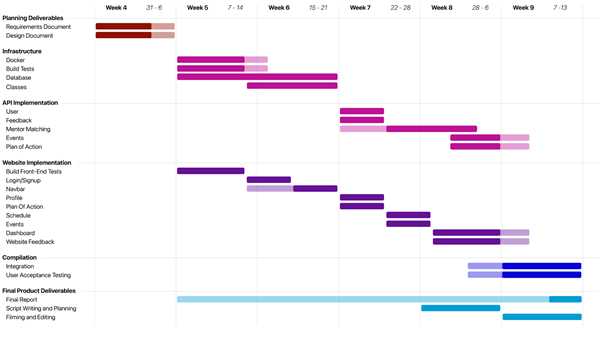
\includegraphics[width=0.75\textwidth]{Timetable}
    \caption{Gantt chart of the project schedule.}
    \label{fig:project_schedule_gantt}
\end{figure}

The timeline outlines which features of the system will be implemented in each
weekly sprint, divided according to the team which is working on them, with
final product documentation separated as this is a collaborative effort by the
whole team. As we are following a Scrum methodology, task order may be adjusted
weekly, ie. in each sprint, so that the project remains on track, so which
features are completed in each week will most likely change. It also acts as a
reminder that the final report should be completed, when time is available,
concurrently with the project itself, so it doesn't need to be written in its
entirety in the few days before submission.


\section{Technical description}

% TODO: Decide whether to drop
\subsection{Scope}
Our system must satisfy a complex specification, so its development must be
carefully planned and executed. However, the goal is to create a prototype, not
a finished product. This means that some features that would be required in
production, which do not fit in the timescale for the prototype, e.g. , or would
require integration from external systems, e.g. company calendar applications,
should not be implemented. Our requirements analysis fully defines the scope of
what we will implement.

\subsection{System attributes}
It is crucial that the system's usability is considered. Our goal is to ensure
that the website is intuitive to use, has little ambiguity and can ideally be
learnt without assistance even by non-technical users. Thorough acceptance
testing will be carried out to ensure this is achieved. Along with this, our
prototype aims to make our system accessible to people with disabilities, by
including features such as enlarging text and higher contrast colours.

Both compatibility and portability are important aspects to consider when
designing a system. As the system is a web app, it is inherently compatible
since every user will have some access to a device able to run a browser.
Furthermore, since websites use standardised languages such as HTML, they are by
definition portable across devices running valid browsers. Extreme cases such as
legacy browsers will not be prioritised since it is unlikely to be used. The
prototype will not include desktop and mobile applications since it would be
difficult to make portable across systems, and so is out of the scope of the
prototype.

Security is also important to consider, especially due to the legal obligations
on processing of user data that grow more stringent over time. It is impossible
to have a system which is both functional and perfectly secure, however, the
threat surface for any prototype system is very small, so it is sufficient to
follow simple best practises, such as account access protection through hashing
and salting stored passwords. Data will only be accessed through the REST API,
allowing us to ensure only required data is sent, and adds a layer of security
since our database is not directly interacted with. Furthermore, it also allows
us to also validate any user information before storing it in the database.

Robustness, reliability and fault tolerance must also be accounted for in the
design. One of the benefits of containerisation in these categories, as if a
fault occurs, the individual container containing the broken component can be
restarted or fixed independently from the rest of the system. This means that
the uptime of the system as a whole is less likely to be damaged, and if it is
it will be down for a shorter period of time.

Modularity and reuse, and extensibility are further important design components.
Modularity is largely implemented by splitting the architecture up into two
sections: the frontend and the backend. These can then be developed largely
separately, relying on a predefined API to communicate with each other, then
integrated together later. This also improves extensibility, for example as new
frontend designs can be added without changing the backend by using pre-existing
API calls.

Correctness is the final aspect which we consider in the design. Correctness of
complex systems is much more arbitrary than of simple algorithms. For example,
an algorithm could be formally proved to always give the correct output given
any input, but a complex system can only be shown to satisfy its requirements.
This is done by comprehensive testing of every component in the system, known as
end-to-end testing - and is discussed in our testing section.


\subsection{Technologies used}

% NEED TO UPDATE THIS TO USE TABLE
A fundamental decision in the project is deciding which technologies should be
used to compose the so-called ``tech stack''. Since this is such an important set
of decisions, we carefully considered a number of options with respect to a set
of criteria which assess the quality of a component technology choice. These
criteria include:
\begin{itemize}[leftmargin=1.2cm,noitemsep,align=left]
    \item
        Suitability, how well does the technology match the problem
        our system solves?
    \item
        Documentation and popularity, does the choice have strong
        documentation and an active community likely to have already answered problems
        we may encounter?
    \item
        Consistency, how well the choice meshes with the other
        component technologies?
    \item
        Performance, will the technology run sufficiently fast,
        and can it be scaled later needing to switch to something else more performant?
    \item
        Experience, how much prior knowledge does our team have of the technology?
\end{itemize}

\begin{longtable}{|p{0.085\linewidth}|p{0.09\linewidth}|p{0.75\linewidth}|}
    \hline \textbf{Category} & \textbf{Choice} & \textbf{Justification} \\ \hline\hline


    Application type
    &
    Web app
    &
    Suitable as it is portable and compatible
    across devices, since it is run in-browser, and can be designed to support
    differing view widths such as mobile. All of the team has experience with
    web design.
    \\ \hline

    Backend framework
    &
    Django
    &
    Suitable as it facilitates fast development, needed for prototyping, and
    inherently supports non-functional requirements of security and scalability,
    and it is popular. Because of this, it has consistent integrations with
    other categories. Based on python, which team has experience with.
    \\ \hline

    Web server
    &
    NginX
    &
    Suitable as it serves static web content effectively, and is an industry
    standard. More performant than its competitor apache. Consistent with Django
    backend in common technology stacks
    \\ \hline

    Frontend framework
    &
    Vue.js and Bootstrap
    &
    Since we are making a web application, we will use HTML/CSS/JS. We decided
    to use the Vue.JS framework to develop the frontend, as it facilitates
    writing responsive websites, but has a much less steep learning curve than
    other frameworks, and is known to integrate well with Django. Using a
    framework, provides us with powerful tools that allow us to develop the
    frontend quicker than if we did this project without it. Furthermore, we are
    going to use bootstrap as the CSS framework as it allows us to quickly
    develop a professional looking website with little hassle.
    \\ \hline

    Database
    &
    PostgreSQL
    &
    Suitable as it is a relational database, which fits the type of data we need
    to store, e.g. user accounts, calendars, etc. and it is popular. It has very
    strong documentation compared to other SQL flavours, It is consistent, as it
    has a good integration with Django. All of the team has experience with it
    from a previous module
    \\ \hline

    API
    &
    JSON REST
    &
    Suitable as it facilitates the access of only the required data. It is
    incredibly ubiquitous, as it is a subset of Javascript, and hence is
    consistent with our Vue.js framework. Both our backend and frontend team
    members have experience with it, which is crucial as it will form the link
    between the two sides of the technology stack
    \\ \hline

    Container- isation
    &
    Docker
    &
    % TODO: ADD REFERENCE https://www.techrepublic.com/article/the-10-most-popular-container-tools-for-businesses/
    Suitable as it is the de-facto standard for containerisation (57\% share),
    so strong documentation and an active community. Consistent with all of the
    other technologies. \\ \hline

    Version control
    &
    git with GitHub
    &
    Suitable as it is full featured, supporting branching for collaboration,
    remote backups, and CI/CD through GitHub actions. Industry standard, so
    strong documentation and an active community. Consistent with all other
    technologies. All of the team has experience with it from a previous module.
    \\ \hline

\end{longtable}

When deciding on our technologies, we considered using some form of machine
learning in the project - specifically for the matching system for mentors and
mentees. However, we decided against doing this for a number of reasons. We
thought that an algorithmic solution would produce better solutions, given the
varied type of metrics that are recorded, and the fact that not enough data
points on what a good match entails would be recorded to adequately train a
model, as mentoring relationships are likely to last years at a time. However,
we did decide to use sentiment analysis on feedback, as more (helpful), data
metrics almost always improves prediction quality of an algorithm. We plan to
use the python library NLTK to implement this, as it is consistent with our
python backend, and an industry standard for this type of application.

\subsection{System architecture}
Our system architecture follows the MVC (Model View Controller) architecture
which is a well-known model to be successful in creating a system that presents
data obtained through a controller that interacts with the database. This is
reflected in the Docker containerisation figure with our website being the view,
the Django system being the controller, and Postgresql as the model. Being
modularised to 3 separate components, allows easy distribution of development,
with each focusing on a subset of skill sets. One downfall of this architecture
is that the system is tightly connected in that if one system fails, the rest
falls - however we believe that this is outweighed by the benefits of this
architecture. Furthermore, the fact that it is a trusted design pattern suggests
it is not an inherently problematic approach. A REST API will be used to serve
data to the user, allowing both static site pages and dynamic JSON data to be
served from the Django backend.

We decided to containerise our model, as the specification stated that Deutsche
Bank already uses containers for this type of application, so it will provide
modularity within their existing systems. Furthermore, it gives the property of
easy ``lift-and-shift'', meaning that all the dependencies can be handled within
the containers, which themselves are portable and compatible across machines.

We decided against using microservices, instead opting for a monolithic
architecture. This was predominantly for two reasons: Django has a higher
overhead than other backend frameworks like Flask, so making multiple
microservices can reduce performance; and there is not a clean way nor a good
reason to split the internal logical model into separate microservices.

When designing our system architecture, we took into account the ``twelve factor
application'' principles. For example using a workflow based around git to fulfil
the codebase and release principles, or using docker to fulfil the dependencies,
and port binding one.

\begin{figure}[H]
    \centering
    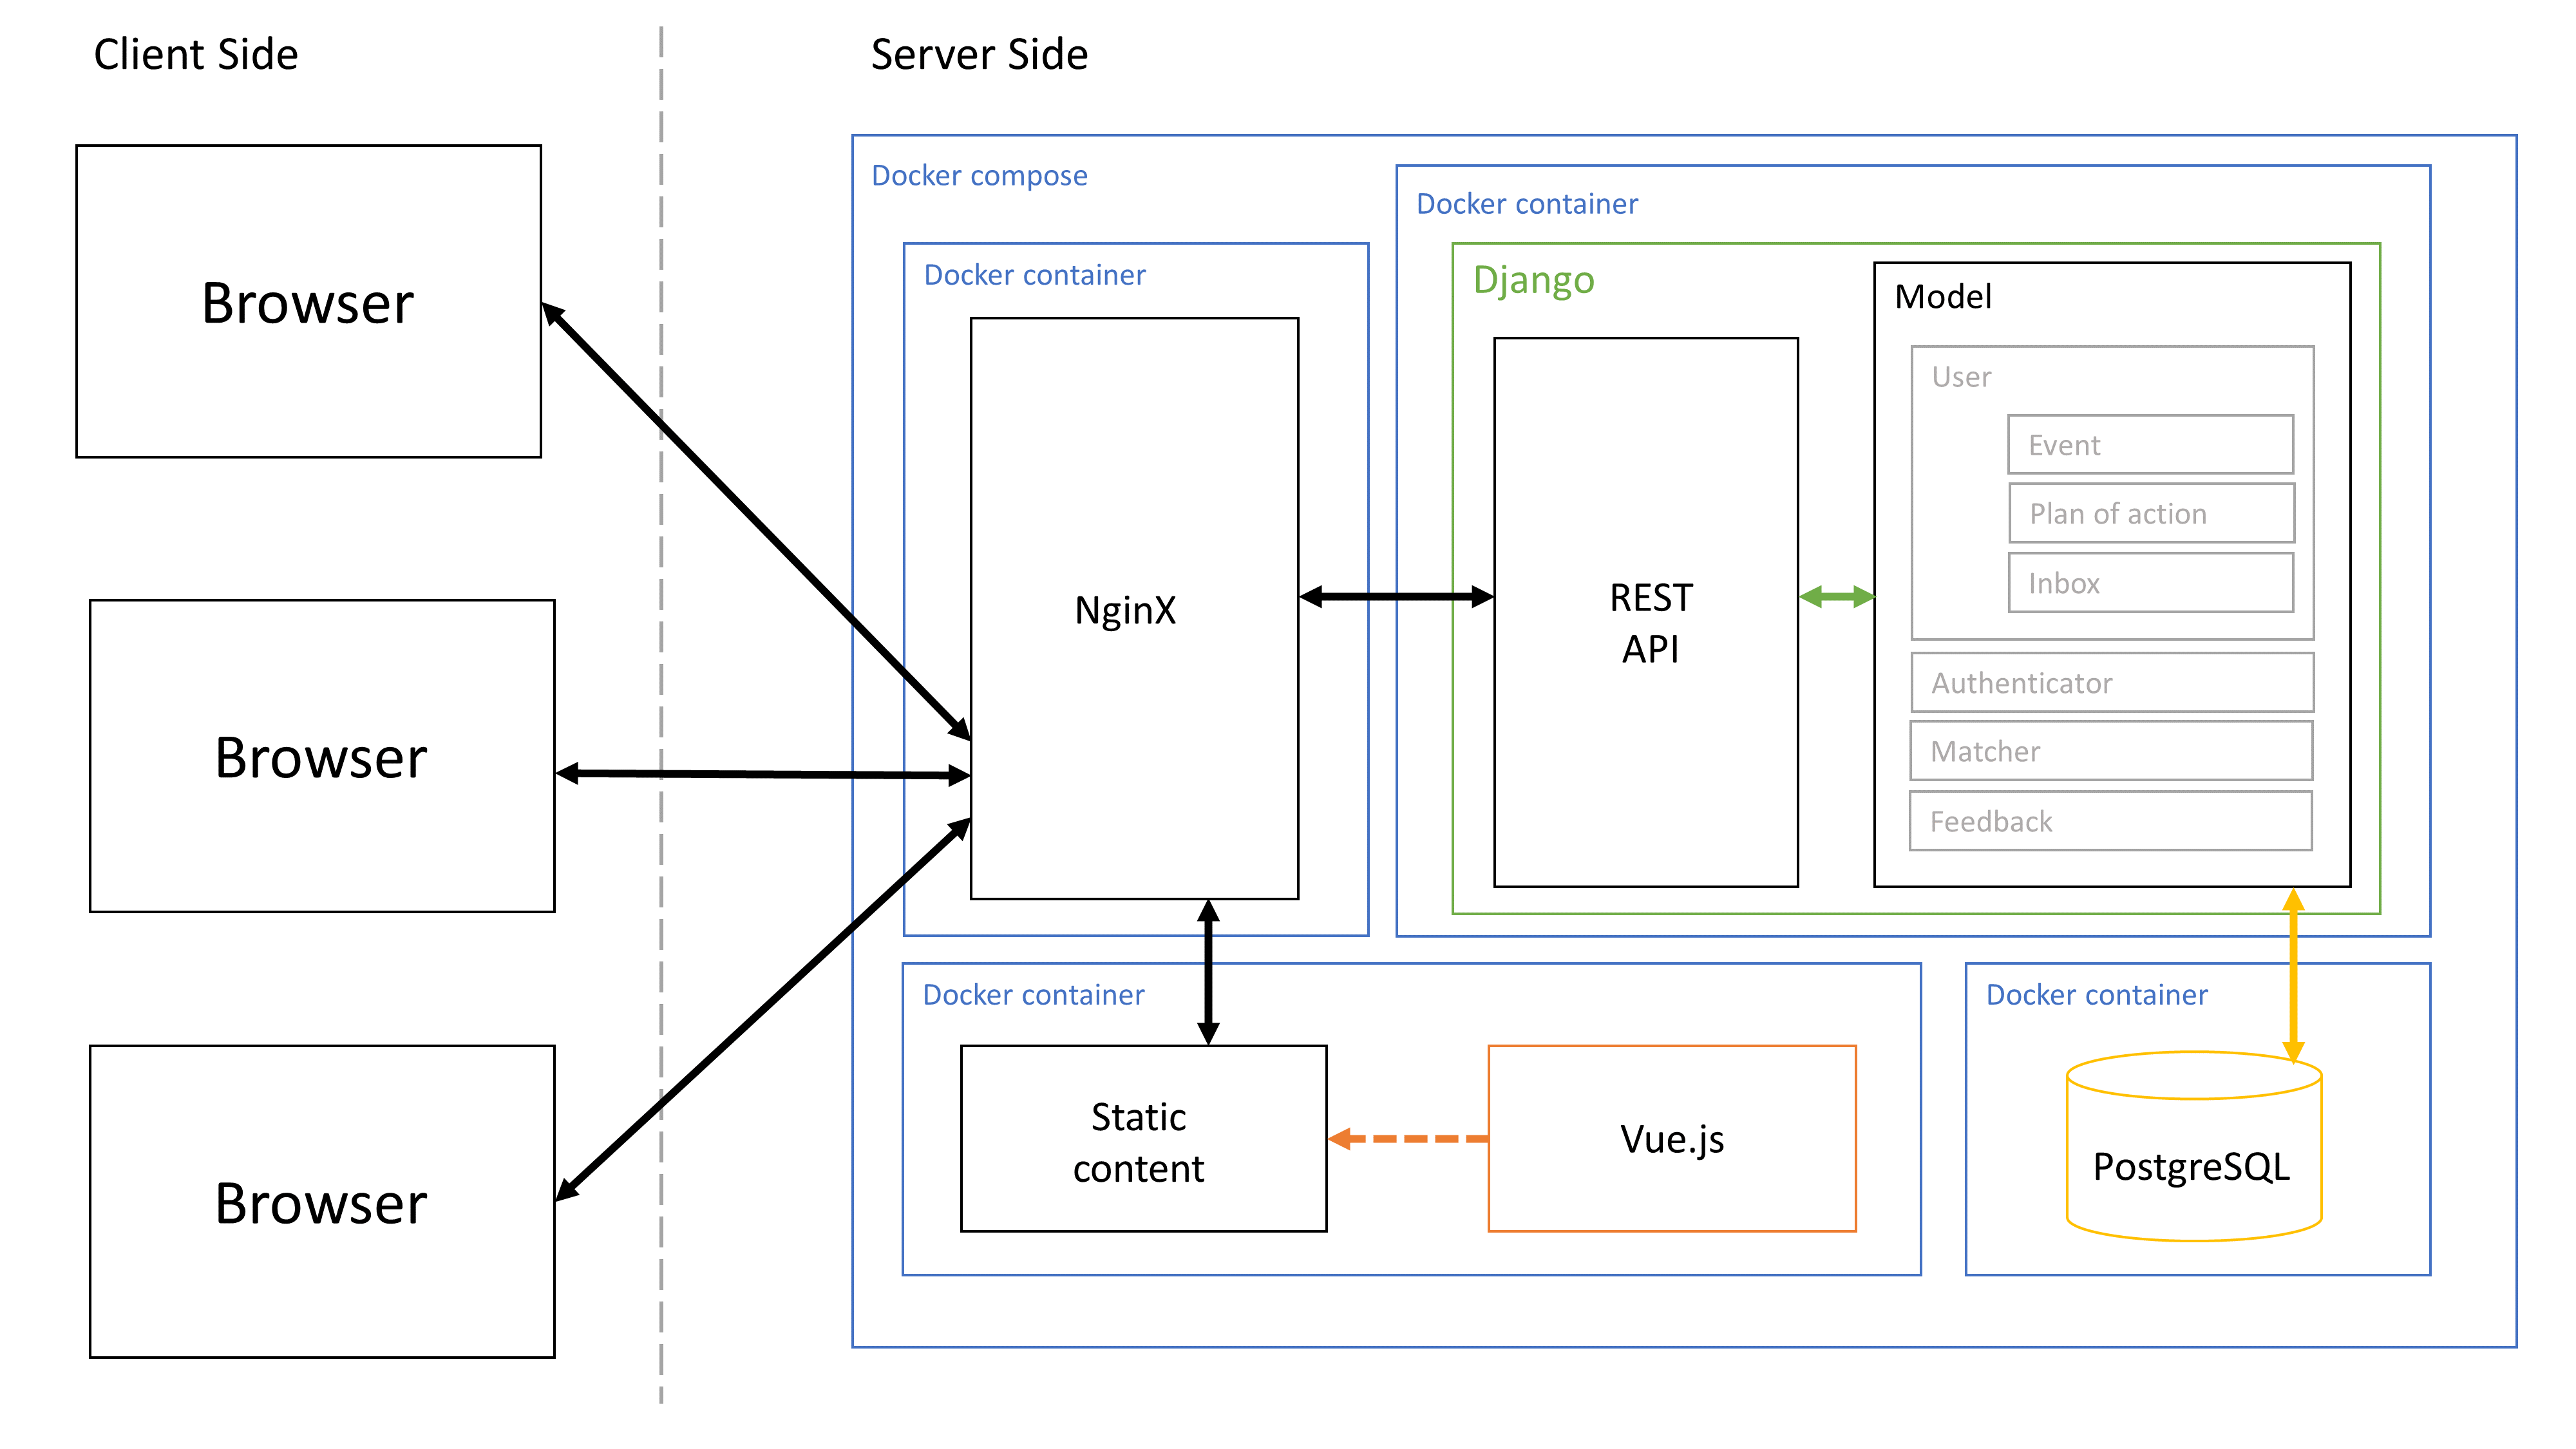
\includegraphics[width=0.75\textwidth]{architecture}
    \caption{A system diagram of our system architecture.}
    \label{fig:system_architecture_diagram}
\end{figure}

The containerisation has two distinct parts. The first is the three containers
dynamically interact with each other based on user requests, with the NginX
container serving requests into the Django backend container, which runs the
internal logic, and can look up data from the postgresql database container. The
second is the final container which generates the static site content from
Vue.js to pure HTML, CSS, and Javascript. This is then copied into the Django
container so it only needs to be generated once, not on a request-by-request
basis.

\subsubsection{Database Design}

The User table stores relevant user information required by the overall system.
BusinessArea and StrengthWeakness tables lists all possible options the user may
choose as it is not free text. PasswordReset should only have unique userIDs to
ensure there is only one reset code, and should be removed if it has expired.
Notifications and Milestones will be searched by userID to obtain a user's
relevant data entries. Authentication stores a token to be matched with what is
stored in the user's cookies to reduce the number of logins as it can be
annoying for users.

Pairing table reflects the current mentor-mentee pairings between users.
Important constraint is that a userID must be unique in the menteeID column
since mentee's can only have one mentor. Event table is different from a meeting
in that it has multiple mentees, a capacity of number of people that can join
and a type - GroupSession or Workshop. ProposeMeeting can only store one
proposition for a meeting at a time relative to a pairing. If the mentor
rejects, it is reflected by a boolean and a note for the mentee.
RejectMentoringOffer is expected to be used in suggestion lists, to temporarily
hide a mentee in the case that mentee rejects a mentoring offer (F08).

Feedback has been decomposed to 4 types. To ensure efficiency and scalability,
each type of feedback has its own table rather than trying to abstract
commonalities, creating dependencies that could be problematic in the future.
The difference between MeetingFeedback and EventFeedback is if it's for a
meeting or event. General Feedback stores overall feedback to a mentor by
mentee. These 3 will store an analysis of its sentiment, that will be used in
the suggestion process. SystemFeedback has two types, error or feature that is
used by developers to improve their system.

\begin{figure}[H]
    \centering
    \subfloat[\centering The user tables schema.]{{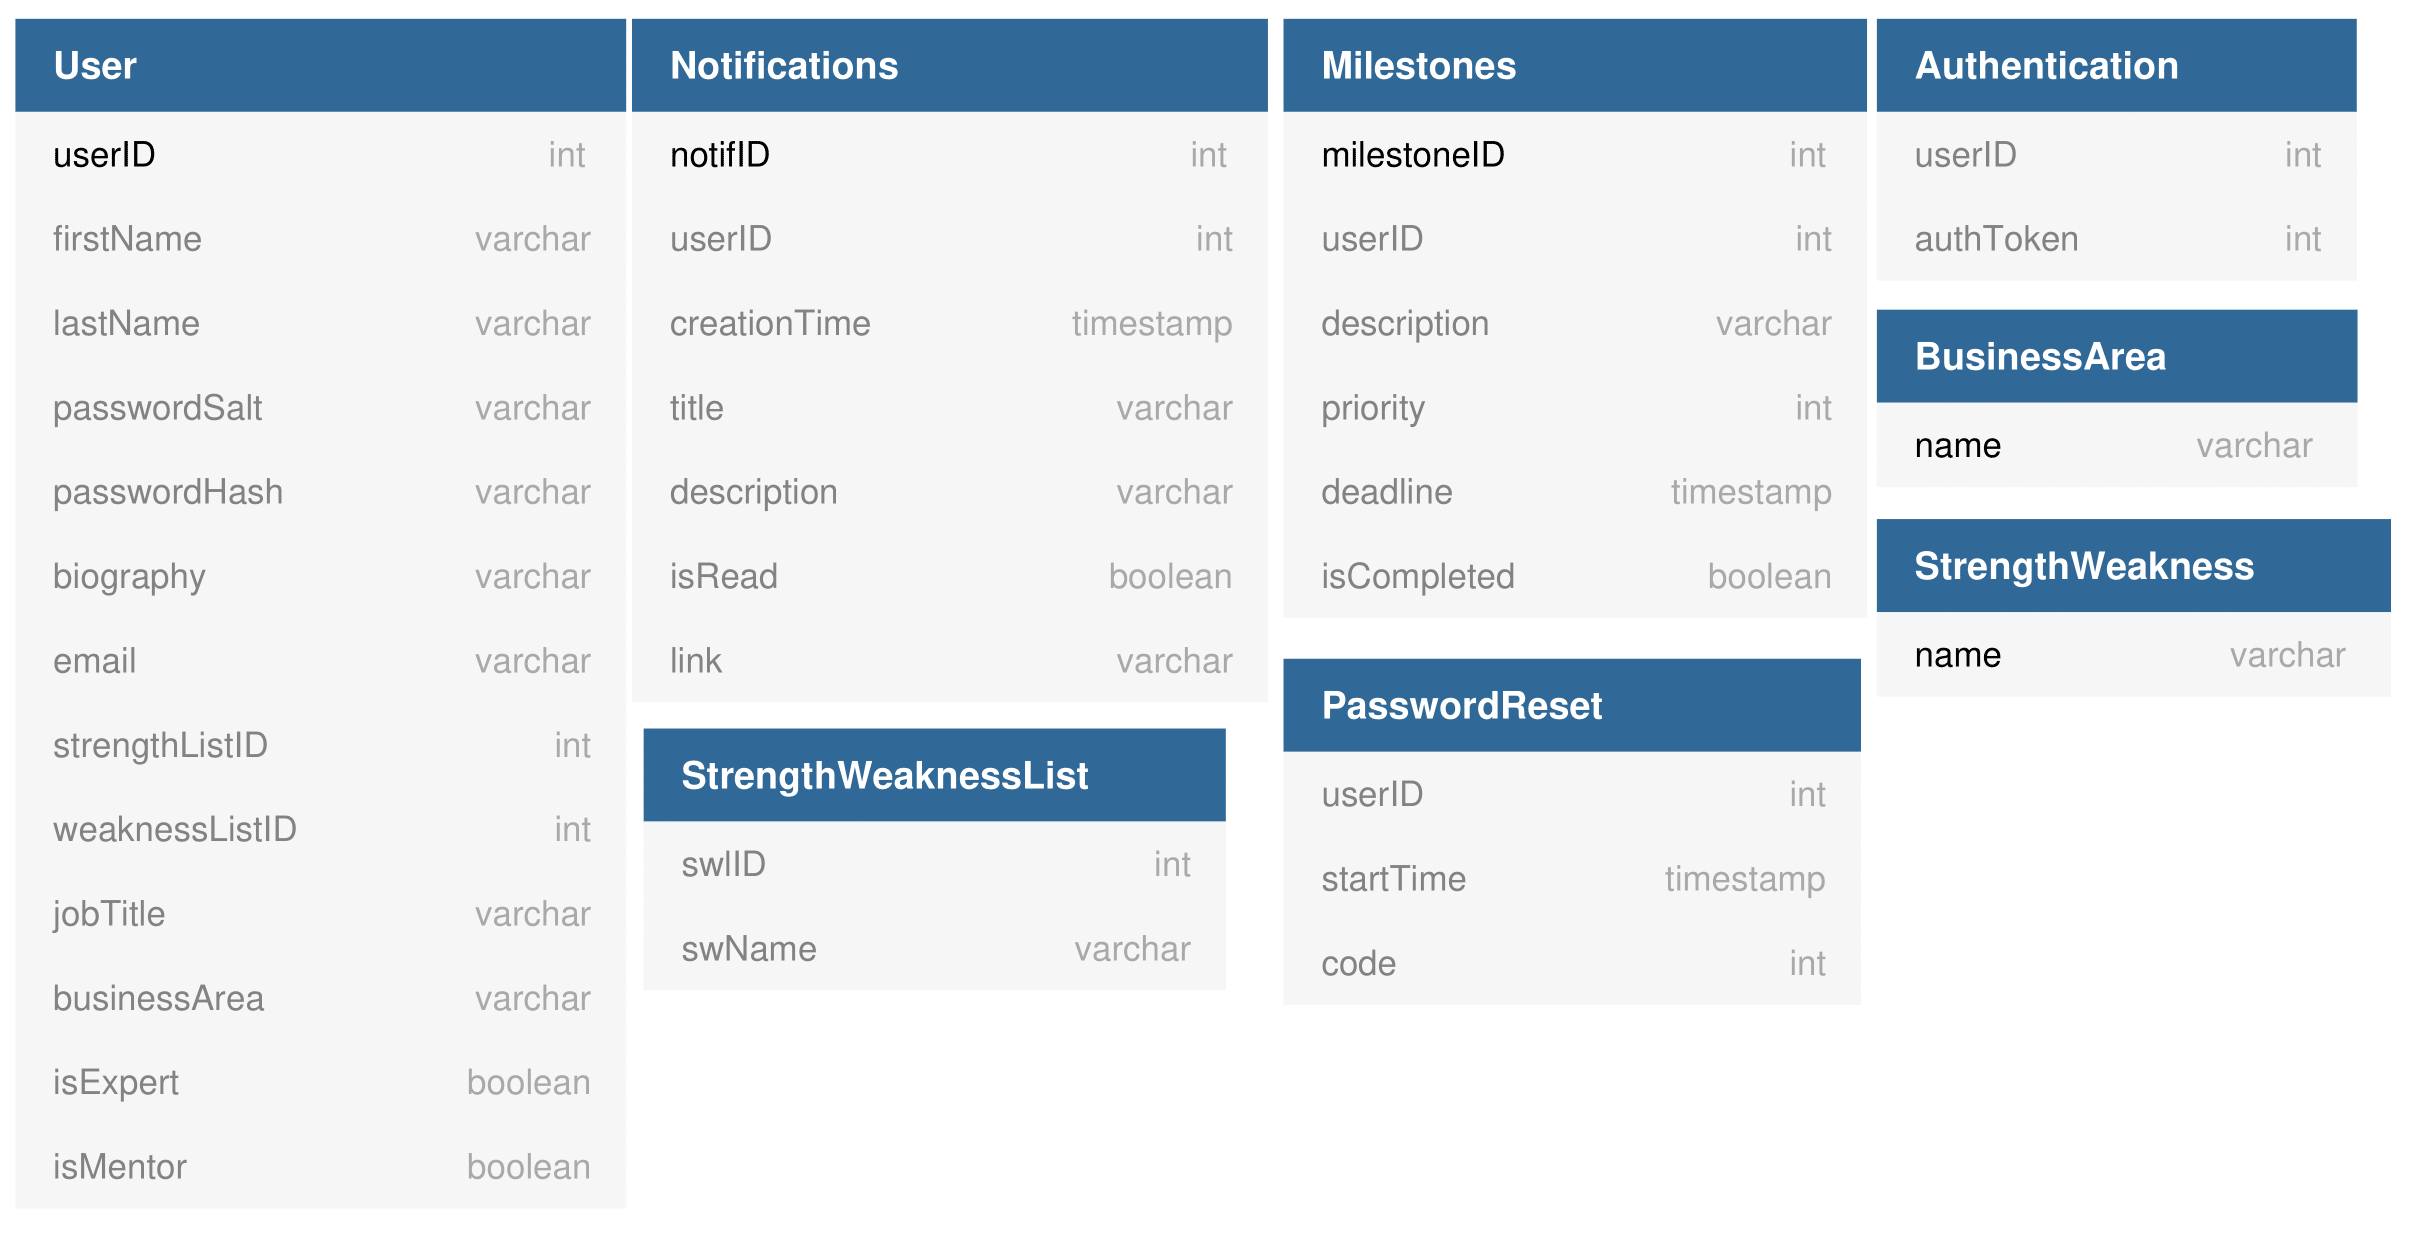
\includegraphics[width=0.45\textwidth]{UserDB} }}
    \qquad
    \subfloat[\centering The mentoring tables schema.]{{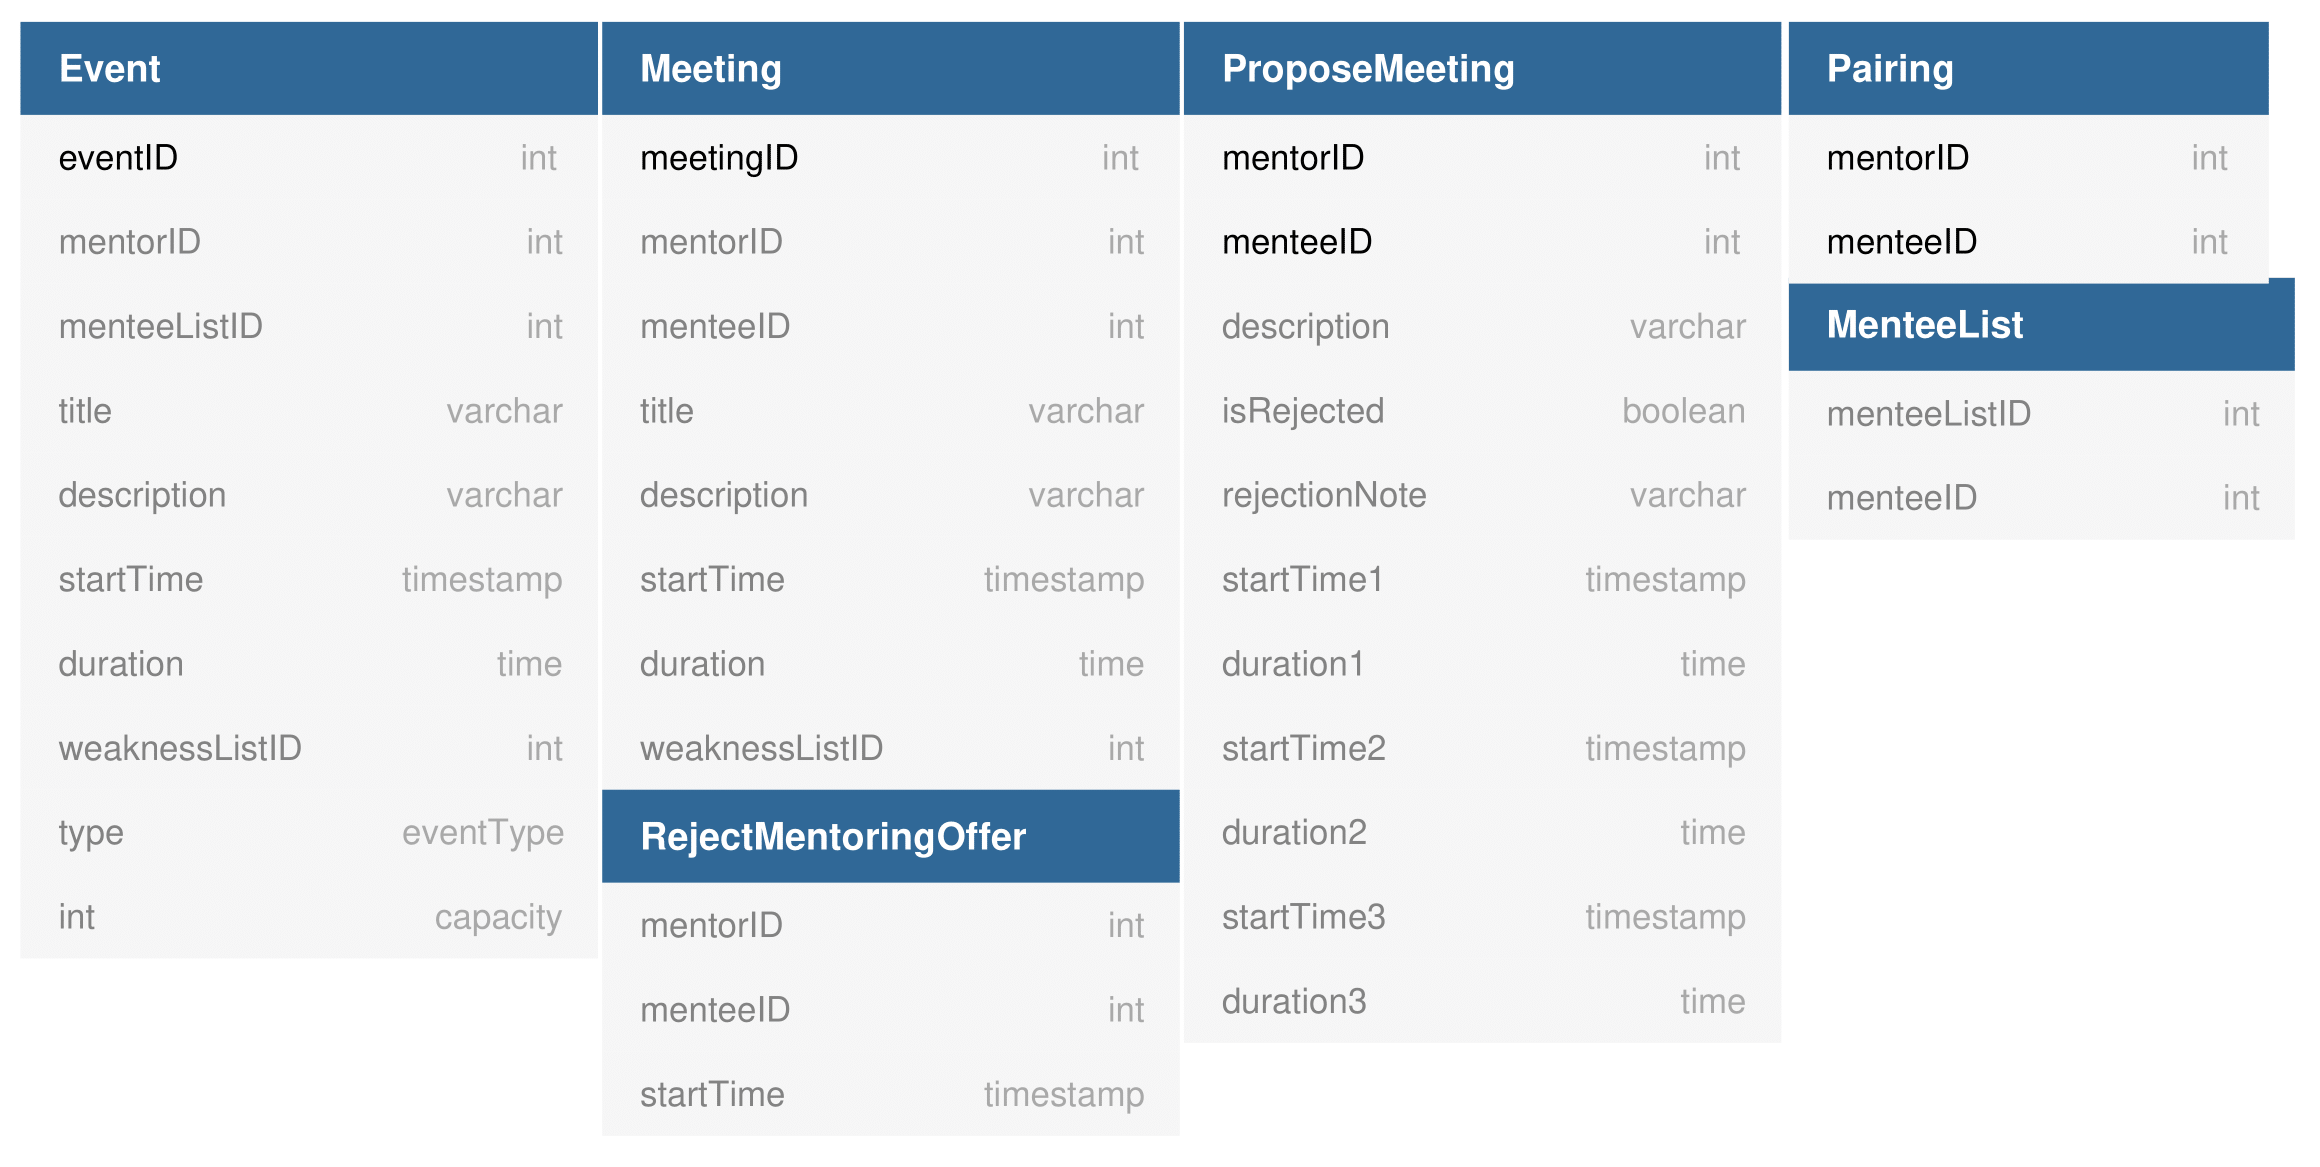
\includegraphics[width=0.45\textwidth]{MentoringDB} }}
    \newline
    \subfloat[\centering The feedback tables schema.]{{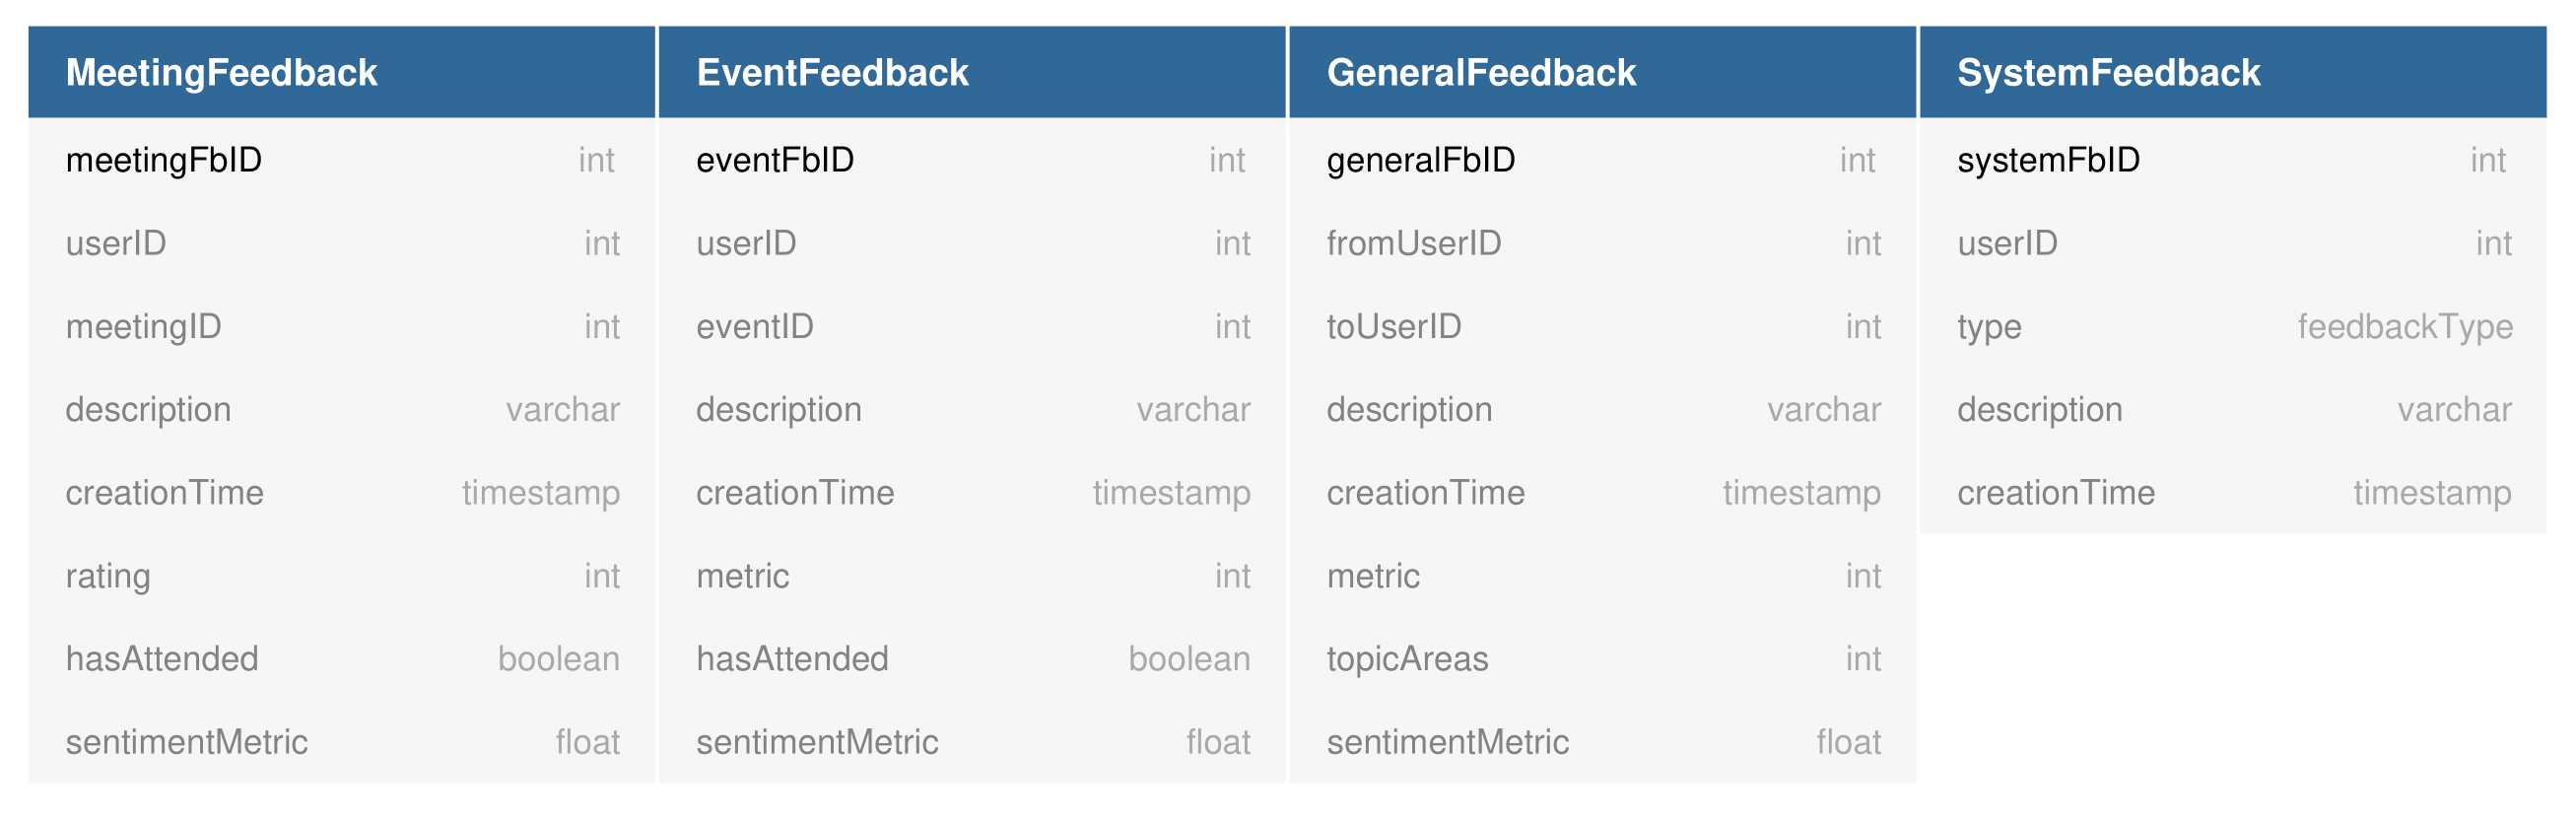
\includegraphics[width=0.65\textwidth]{FeedbackDB} }}
    \caption{Table schemas of groups within our systems' database schema}
    \label{fig:db_entity_relationship}
\end{figure}

% \begin{figure}[H]
%     \centering
%     \subfloat[\centering The feedback tables schema.]{{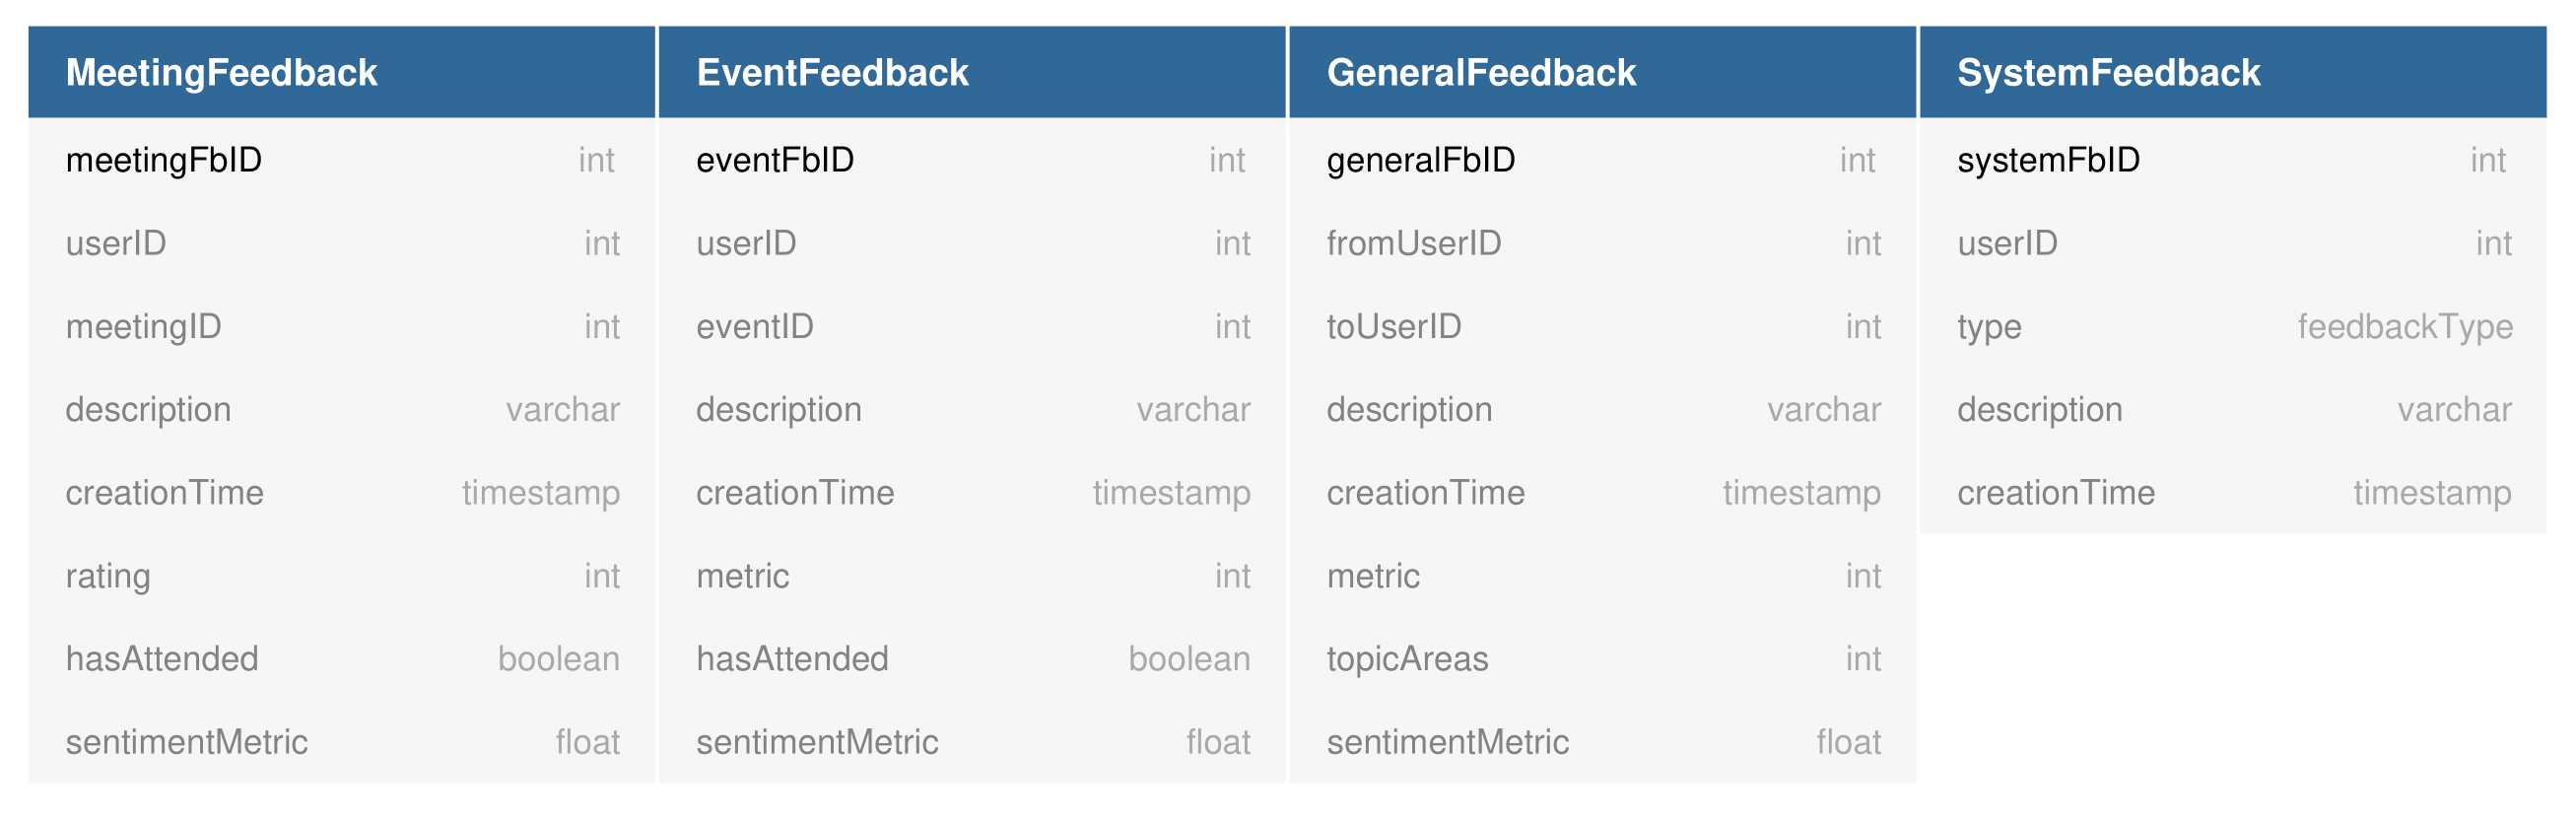
\includegraphics[width=0.5\textwidth]{FeedbackDB} }}
%     \qquad
%     \subfloat[\centering The entity relationship for the database.]{{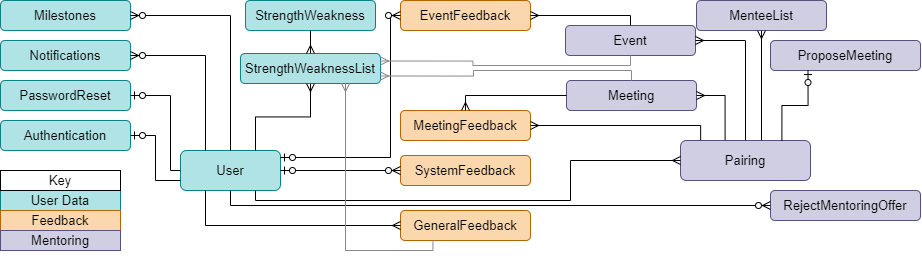
\includegraphics[width=0.75\textwidth]{ER} }}
%     \caption{Table schemas and entity relationship diagrams for the tables in the database schema}
%     \label{fig:db_entiry_relationship}
% \end{figure}


% \begin{figure}[H]
%     \centering
%     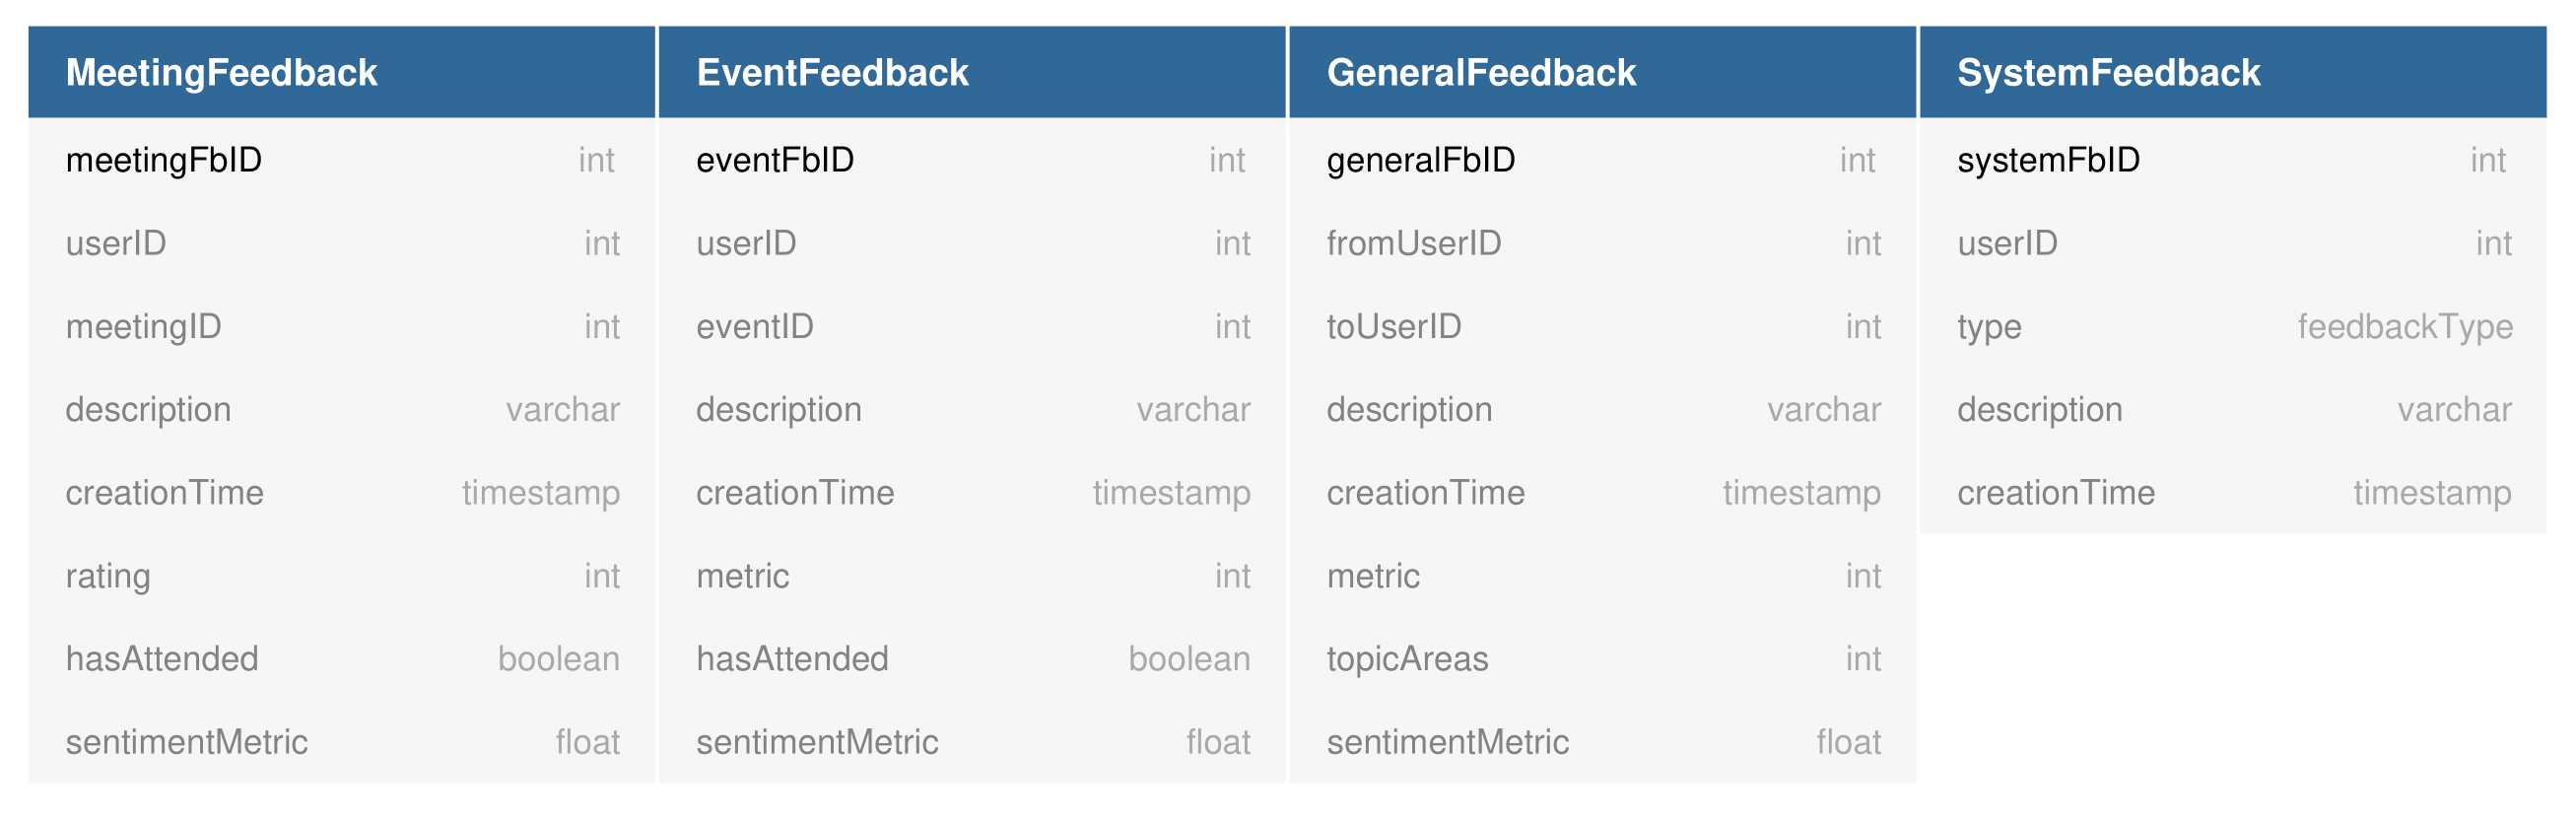
\includegraphics[width=0.55\textwidth]{FeedbackDB}
%     \caption{The feedback tables schema.}
%     \label{fig:Feedback_Schema}
% \end{figure}

The three subgroups shown in the above figures all relate to each other in the
way shown in the final figure. This is done to make the complex schema more
easily parsable, whilst retaining detail.

\begin{figure}[H]
    \centering
    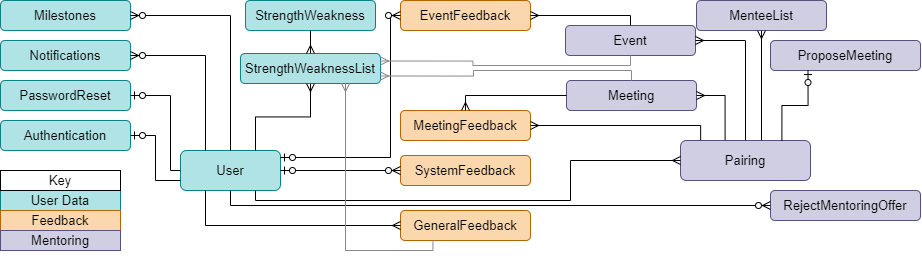
\includegraphics[width=1\textwidth]{ER}
    \caption{Entity Relationship Diagram.}
    \label{fig:Entity Diagram}
\end{figure}


\subsubsection{Object Structure}
We've decided to take an object oriented approach on the back-end side of the
application. This allows us to separate the problem into multiple smaller
subproblems which can be solved one at a time. It also allows for different team
members to work on different sections of the back-end code simultaneously, thus
improving our team's efficiency; each back-end developer will be assigned a set
of classes which can be worked on independently. As shown in the class diagram,
we've utilised inheritance wherever suitable. This reduces the complexity of the
problem, and means that we'll have to write less code overall, therefore saving
time for our backend developers—something that is especially important when
considering the short timescale of the project. The object oriented approach is
particularly useful when trying to model the problem as a whole. The use of
techniques such as aggregation and composition, help model the relationships
between objects in the system, giving us a greater understanding of how data
will flow.

% TODO: CHECK ; Believe I have updated this to the most recent one
\begin{figure}[H]
    \centering
    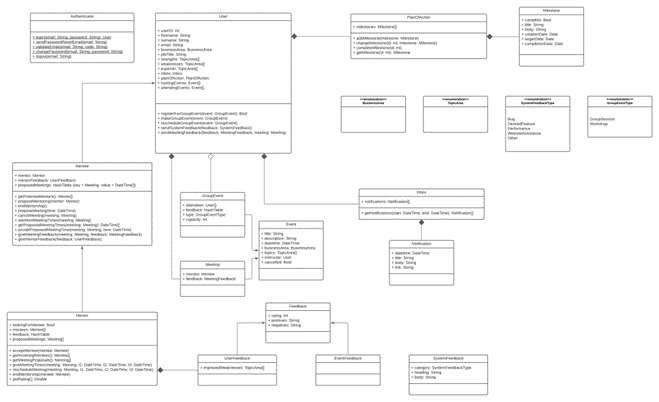
\includegraphics[width=1\textwidth]{Objects}
    \caption{A UML class diagram of our object structure.}
    \label{fig:uml_class_diagram}
\end{figure}


\subsubsection{API design}
We have planned to design an API which will be used by the front-end to
interface with the core back-end components of the system. We've decided to
settle on a REST API implementation, as it emphasises client-server decoupling,
which will make it easier to separate front-end and back-end tasks between our
developers—something which is of the utmost importance when working in a
smaller, less experienced team. The REST API system will give the front-end
developers access to fixed API endpoints, which will act as a bridge between the
front-end and back-end of the application. The front-end developers won't need
to know how these endpoints are implemented, they only need to know what
functionality they provide. This will save development time as developers can
now focus on their specialties. This modular way of designing the API allows for
back-end code to be modified without having to consult the front-end developers
about potential consequences. As long as the specification is followed, a
back-end modification should have no effect on how the front-end developers
interact with the system. Overall, this will save time as unnecessary
communication between developers will be eliminated.


\begin{longtable}{|p{0.128\linewidth}|p{0.08\linewidth}|p{0.75\linewidth}|}
    \hline \textbf{Resource} & \textbf{HTTP method} & \textbf{Description} \\ \hline\hline
    register
    &
    POST
    &
    Registers the user. A newly created user ID is sent in the response payload. A session ID will be in the response header, to be stored as a cookie.
    \\ \hline

    login
    &
    POST
    &
    Logs the user into the application if the email and password match. The user ID is sent in the response payload. A session ID will be in the response header, to be stored as a cookie.
    \\ \hline

    resetPassword
    &
    PUT
    &
    Resets a user's password.
    \\ \hline

    getProfile
    &
    GET
    &
    Asks the server for a user's profile information (user ID will be specified). The profile information is then sent back in the response payload.
    \\ \hline

    getPotential- Mentors
    &
    GET
    &
    Gets a list of potential mentors for the mentee.
    \\ \hline

    selectMentor
    &
    POST
    &
    Indicates that the mentee wants to be mentored by a particular mentor from the list of potential mentors.
    \\ \hline

    getRequested- Mentees
    &
    GET
    &
    Gets a list of mentees which have requested to be paired with a particular mentor.
    \\ \hline

    acceptMentee
    &
    POST
    &
    Used by a mentor to indicate that they want to begin a relationship with a particular mentee.
    \\ \hline

    getMentor
    &
    GET
    &
    Gets the mentor of a particular mentee.
    \\ \hline

    getMentees
    &
    GET
    &
    Get a list of the mentor's mentees.
    \\ \hline

    terminateRel- ationship
    &
    DELETE
    &
    Terminates a mentoring relationship. Feedback for termination is provided in the request.
    \\ \hline

    proposeMeeting
    &
    POST
    &
    Allows the mentee to propose a meeting.
    \\ \hline

    proposeMeeting- Times
    &
    POST
    &
    Allows the mentor to send a list of potential meeting times back to the mentee.
    \\ \hline

    acceptMeeting
    &
    POST
    &
    Allows the mentee to accept one of the meeting times proposed by the mentor.
    \\ \hline

    reproposeMeet- ing
    &
    POST
    &
    Allows the mentee to ask for new meeting times.
    \\ \hline

    cancelMeeting
    &
    DELETE
    &
    Gives feedback for a particular meeting.
    \\ \hline

    getMeetings
    &
    GET
    &
    Get a list of scheduled meetings.
    \\ \hline

    giveMeeting- Feedback
    &
    POST
    &
    Gives feedback for a particular meeting.
    \\ \hline

    getPlanOfAction
    &
    GET
    &
    Get details of the plan of action.
    \\ \hline

    addMilestone
    &
    POST
    &
    Adds a milestone to the plan of action.
    \\ \hline

    setMilestone
    &
    PUT
    &
    Changes the content of a milestone.
    \\ \hline

    completeMile- stone
    &
    POST
    &
    Set a particular milestone to complete.
    \\ \hline

    getMilestone
    &
    GET
    &
    Get information about a particular milestone.
    \\ \hline

    setMentorFeed- back
    &
    PUT
    &
    Allows a mentee to update their current feedback on their mentor.
    \\ \hline

    createGroup- Event
    &
    POST
    &
    Allows a mentor to create group sessions or workshops. The type of event is specified in the request.
    \\ \hline

    getGroupEvent
    &
    GET
    &
    Get details about a particular group session or workshop.
    \\ \hline

    joinGroupEvent
    &
    POST
    &
    Allows a user to sign up for attending a group event.
    \\ \hline

    getNotifications
    &
    GET
    &
    Gets notifications for a users' inbox, with the date range being specified.
    \\ \hline

    submitSiteFeed- back
    &
    POST
    &
    Allows users to give feedback about the site.
    \\ \hline



\end{longtable}




\section{UI/UX design}

\subsection{Page Hierarchy}
The page hierarchy below displays the sites that our webpage comprises of. Here
is a brief outline of what each page will consist of:

\begin{figure}[H]
    \centering
    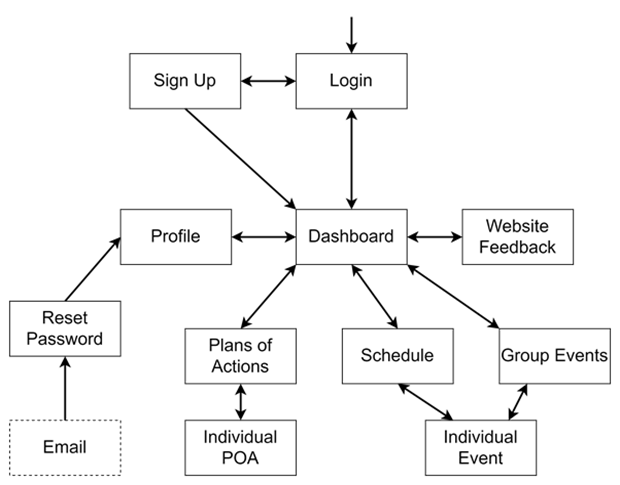
\includegraphics[width=0.55\textwidth]{Hierarchy}
    \caption{A diagram of website page hierarchy.}
    \label{fig:website_page_hierarchy}
\end{figure}

\begin{itemize}[leftmargin=1.2cm,noitemsep,align=left]
    \item Login Screen: The landing page of the website that allows the user to
    login to go to the dashboard or the sign up page to create an account.
    \item Sign Up: Allows the user to create an account.
    \item Dashboard: The central hub for the user where all pages can be
    accessed from and displays useful information that may be useful (look at
    page designs for more detail).
    \item Profile: This page has 3 purposes: resetting the users password,
    seeing the users data and modifying the users data.
    \item Plans of Action: Displays the users plan of action and their mentees
    plans of actions too if they have any.
    \item Individual POA: If the user clicks on a POA, then they come to this
    page where the POA can be viewed and modified.
    \item Schedule: Shows the users schedule, allows them to request meetings
    and has a list of feedback and meeting requests that the user should respond
    to.
    \item Group Events: Allows the user to search for workshops and group
    sessions within the system that they can attend.
    \item Individual Event: A page that details an event (meeting or group
    event) and allows the owner of an event to modify or delete the event.
\end{itemize}






\subsection{User-system interaction}

\begin{figure}[H]
    \centering
    \subfloat[\centering A diagram of the states required to match a mentor and a mentee.]{{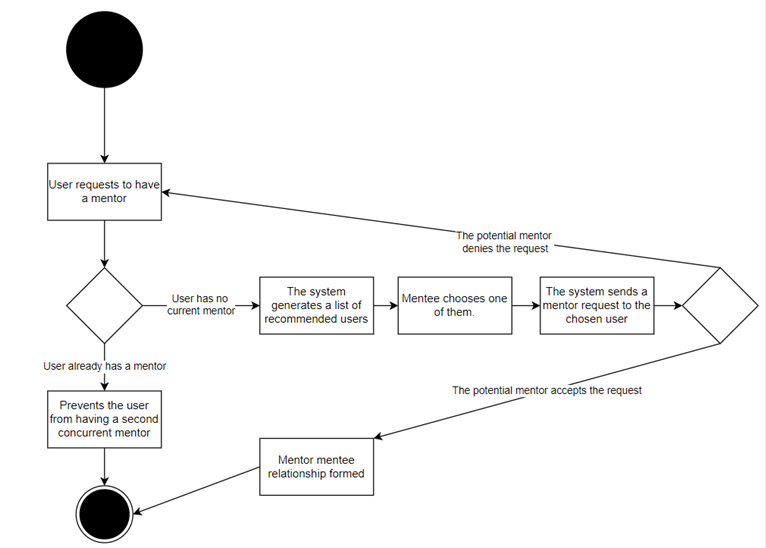
\includegraphics[width=0.45\textwidth]{MentorMentee} }}
    \qquad
    \subfloat[\centering A diagram of the states required to schedule a meeting.]{{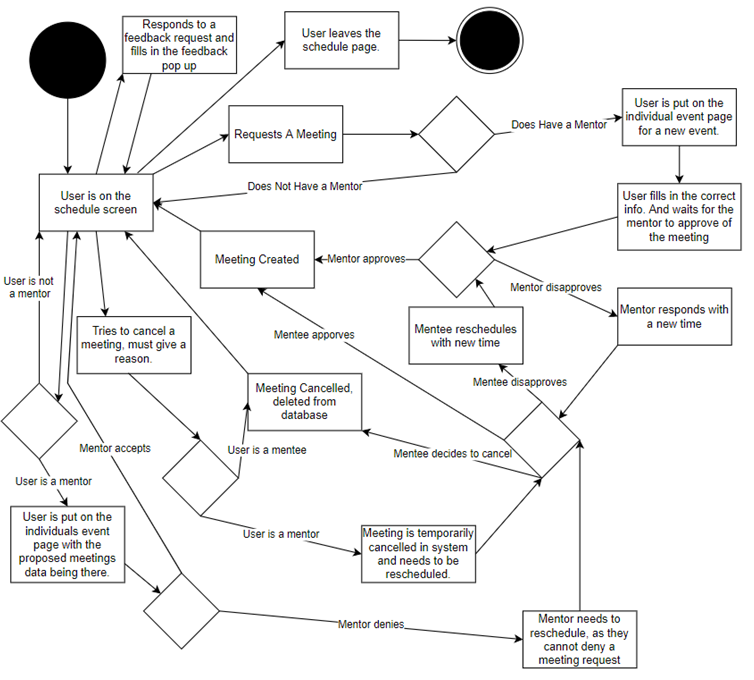
\includegraphics[width=0.45\textwidth]{Meeting} }}
    \caption{State diagrams for some aspects of our design.}
    \label{fig:state_diagrams}
\end{figure}

The specification was very vague about how to match up mentors and mentees. The
left diagram provides a visual representation of how exactly we interpreted it
in our requirements.
\begin{itemize}[leftmargin=1.2cm,noitemsep,align=left]
    \item The user can only have 1 mentor at a time
    \item The system can give the user a list of potential other users who are currently looking for mentees
    \item The user then picks one of these users and a mentor mentee request is sent to the potential mentor
    \item If the potential mentor accepts, then a relationship is formed
    \item Otherwise, the mentee needs to choose another mentor from the list
\end{itemize}

The right diagram displays what functions the Schedule page has. This handles a
lot of ambiguities around how the meeting and feedback system will work within
our system.
\begin{itemize}[leftmargin=1.2cm,noitemsep,align=left]
    \item Mentees can cancel meetings, but mentors can only reschedule
    \item Mentees can request a meeting, but mentors cannot not
    \item For a meeting to be officially approved, both parties need to agree on the time and date otherwise they go into this loop of suggesting times to each other
    \item The user will be prompted on the schedule page to give feedback to recent events they have gone to
\end{itemize}



\subsection{Page Design}
\begin{figure}[H]
    \centering
    \subfloat[\centering The initial design of our system dashboard.]{{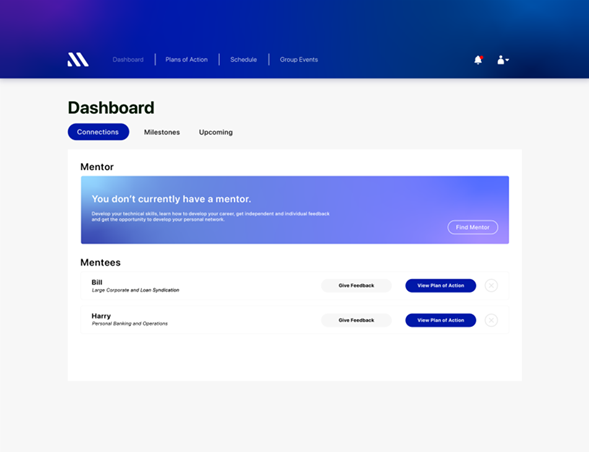
\includegraphics[width=0.45\textwidth]{Dashboard} }}
    \qquad
    \subfloat[\centering The initial design of our system schedule page.]{{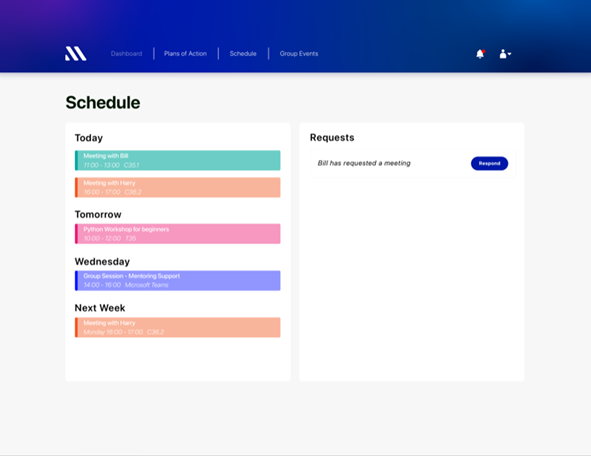
\includegraphics[width=0.45\textwidth]{Schedule} }}
    \caption{Pages from our initial UI designs}
    \label{fig:ui_designs}
\end{figure}

The dashboard is the central page for users that displays all the useful
information for the user, such as their upcoming meetings, their current plan of
action and allows them to get a new mentee or mentor. The navigation bar at the
top of the page will be on most of the pages and will allow the user to access
all the other pages of the website as well as their notifications. The
notifications inform the user about any recent events that they may be
interested in such as giving feedback about a recent event or a mentee/mentor
meeting coming up. The drop down button next to the notification bell will link
to the user's profile page, the website feedback form and a sign out button.

The schedule page will have the users calender and all the requests the user has
(meeting and feedback). This user is not a mentee so the request meeting button
at the bottom is currently missing, but if the user was a mentee then there
would be a request meeting button at the bottom. Additionally, clicking on a
meeting will take the user to the individual event page for the meeting which
will have the feedback log for the meeting.



\section{Testing}
\subsection{Test cases}


\begin{longtable}{|p{0.45\linewidth}||p{0.45\linewidth}|}
    \hline \textbf{Test cases} & \\ \hline\hline

    C0. Verify that the user will be able to create an account by providing correct details; which would be added to the database.
    &
    C15. Verify that general feedback when given is stored into the database.
    \\ \hline

    C1. Verify that the user will be prompted to begin the tutorial for the website.
    &
    C16. Verify if there are sufficient users with common weaknesses, an expert will be prompted to create an event.
    \\ \hline

    C3. Verify that the user can change their password via email, after which it would update their details on the database.
    &
    C17. Verify that events can be viewed by users with relevant weaknesses on their home page.
    \\ \hline

    C4. Verify that users can access and make changes to their profile through their profile page.
    &
    C18. Verify that feedback can be provided at the end of an event.
    \\ \hline

    C5. Verify if making changes to the profile page that breaks a rule of mentoring will prompt a warning that if the change is made the termination of the user's 
    &
    C19. Verify that security issues are disclosed to the users.
    \\ \hline

    C6. Verify that users can request for a mentor by checking if an available mentor can see said mentee of their list of pairable mentees.
    &
    C20. Verify that the widgets on the home page's dashboard navigates the website as intended.
    \\ \hline

    C7. Verify if mentors can fully view the profile of the mentees that are available to pair.
    &
    C21. Verify that the system is intuitive to use and navigate.
    \\ \hline

    C8. Verify if the list is ordered according to the matching metric.
    &
    C22. Verify that it is simple for users with no prior technical experience to use the system.
    \\ \hline

    C9. Verify the mentor can likewise send an offer to a requesting mentee if they would like to establish a pairing.
    &
    C23. Verify that the system is responsive and has no notable or unnecessary waiting time.
    \\ \hline

    C10. Verify that a prompt should be visible when a mentor does not have a mentee.
    &
    C24. Verify that the system can cope with a large number of users.
    \\ \hline

    C11. Verify if mentees can propose a meeting to which a mentor can suggest possible meeting times or which mentees can accept or decline.
    &
    C25. Verify that system changes made by developers are visible within a reasonable time.
    \\ \hline

    C12. Verify if feedback is prompted at the end of the meeting and is stored in the database.
    &
    C26. Verify that the system clears all unit and integration tests.
    \\ \hline

    C13. Verify that mentees can create plans of actions which are then saved on the 'Plans of Action/Milestones' page.
    &
    C27. Verify that the system is secure and protects the users data.
    \\ \hline

    C14. Verify that mentors can access and view any of their mentees' plans of action.
    & \\ \hline

\end{longtable}



\subsection{Unit and integration testing}
Tests will form an integral part of our development cycle, as we plan to follow
the agile test driven development ideologies. We will implement this by creating
unit tests for all of the above test cases, allowing us to ensure all the
required properties of the system are met. These can then be run throughout the
development process. All of the tests will be automatically run on a pull
request to the GitHub repository, and must pass in order for the code to be
merged into the main branch, to ensure its validity. This is an implementation
of ``continuous integration'' from CI/CD, and will be implemented using GitHub
Actions.

There are many tools for unit testing which can be used. Since we are using a
python backend framework, we will use `PyTest' for unit tests on the backend
code, along with `codecov' to assess the coverage of the tests, and `pylint' to
ensure that stylistic code is being written. Since we are using a javascript
frontend framework, we will use `Jest' for unit tests on the frontend code and
UI, along with `ESLint' to check that the Javascript is correct. Finally, we
will use Postman to test that the API serves the correct data. There are
relatively few tools for integration testing, and it will likely mostly have to
be done by hand. We will use the `Puppeteer' tool to automate this task as far
as possible. The combination of all of these tools allows us to create a testing
suite which will fully cover our system.


\bibliographystyle{ieeetr}
\bibliography{designDocument.bib}


\end{document}
